% p10-03 例 1：正方形 ABCD 边长 4，E 是 AB 中点，P 在 BD 上，求 PA+PE 最小
% A 关于 BD 的对称点是 C；最优 P=CE 与 BD 交点
\documentclass[tikz,border=4pt]{standalone}
\usepackage{ctex}
\usepackage{amsmath}
\usetikzlibrary{calc, arrows.meta}
\begin{document}
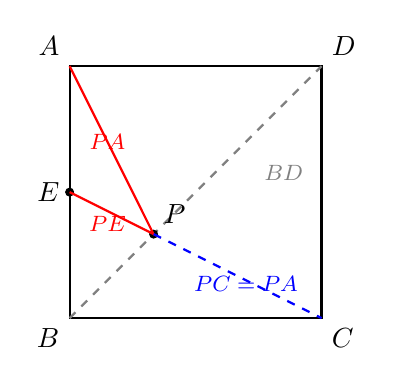
\begin{tikzpicture}[scale=0.8, thick]
  \coordinate (A) at (0, 4);
  \coordinate (B) at (0, 0);
  \coordinate (C) at (4, 0);
  \coordinate (D) at (4, 4);
  \coordinate (E) at (0, 2);   % AB 中点
  % BD 是从 B(0,0) 到 D(4,4)，方程 y=x
  % CE：从 C(4,0) 到 E(0,2)；与 y=x 交点：x=t, y=t；CE 参数 (1-s)(4,0)+s(0,2)=(4-4s, 2s)；y=x ⇒ 2s=4-4s ⇒ s=2/3 ⇒ P=(4/3, 4/3)
  \coordinate (P) at (1.333, 1.333);

  \draw (A)--(B)--(C)--(D)--cycle;
  \draw[gray, dashed] (B)--(D);

  \filldraw (E) circle (1.5pt);
  \filldraw (P) circle (1.5pt);

  % PA + PE
  \draw[red, thick] (A)--(P)--(E);
  % PC = PA (对称)
  \draw[blue, dashed, thick] (P)--(C);

  \node[above left]  at (A) {$A$};
  \node[below left]  at (B) {$B$};
  \node[below right] at (C) {$C$};
  \node[above right] at (D) {$D$};
  \node[left]        at (E) {$E$};
  \node[above right] at (P) {$P$};

  \node[red, font=\footnotesize] at (0.6, 2.8) {$PA$};
  \node[red, font=\footnotesize] at (0.6, 1.5) {$PE$};
  \node[blue, font=\footnotesize] at (2.8, 0.55) {$PC=PA$};
  \node[gray, font=\footnotesize] at (3.4, 2.3) {$BD$};
\end{tikzpicture}
\end{document}
